
The concept of the time has been widely studied \cite{Benthem1982}, \cite{Shackle1961}, \cite{Klein1994}. Moreover, humans beings manage temporal indications in an imprecise way \cite{Devos1998}. But when dealing with time in an Information System, some simplifications must to be done. The first thing to do is the discretization of the time line into time points or time intervals. Both approaches have been proved to be equivalent, although due to the nature of the smallest unit of time in a computer, a \emph{chronon}, the discretization of a time point returns a time interval.

All the possible positions between two time intervals were studied by Allen \cite{Allen1983}, \cite{Allen1985}. As result, the thirteen Allen's Relations were obtained (See Table \ref{tab:allen-relations}) which are illustrated in Figure \ref{fig:allen-relationships}. In order to achieve a more intelligent processing of time, some theoretical frameworks are used to reason with time. First the possibility theory was employed in the reasoning with temporal information \cite{Dubois2003a}. Then, several proposals \cite{Schockaert2008}, \cite{nagypal2003}, \cite{Ohlbach2004}, \cite{Pons2011} studied how to extend the thirteen Allen's relations to the possibilistic case. Also rough set theory \cite{Pawlak1995} has been used to represent and reason about imperfect time intervals \cite{Qiang2009}, \cite{Qiang2010}.

Although there exists several proposals to represent and visualize imperfect time intervals, in this paper we will focus on two: the ill-known constraint framework \cite{Pons2011} and the triangular model \cite{DeTre2012}. The first one is a theoretical framework that deals with temporal reasoning and the second one is a visual framework that represent imperfect time intervals in a two dimensional space. Both frameworks can be used to represent imperfect time intervals as well as temporal reasoning.

The structure of this paper is the following. Section  \ref{sec:preliminaries} introduces the Ill-known constraint framework. Section \ref{sec:triangular-model} introduces the triangular model. Section \ref{sec:proposal} analyze both frameworks and shows the correspondences and differences between both frameworks. The section concludes with an example showing that the calculations made in both frameworks are equivalent. Finally, Section \ref{sec:conclusions} presents the main conclusions and the future work. 


\begin{table}[h]
\centering
\begin{tabular}{|c|l|}
\hline
Name & Implementation \\ \hline 
$I$ equals $J$ & if $s_i = s_j \wedge e_i = e_j $ \\
$I$ starts $J$ & if $s_i = s_j \wedge e_i < e_j $ \\
$I$ started by $J$ & if $s_i = s_j \wedge e_i > e_j $ \\
$I$ finishes $J$ & if $s_i > s_j \wedge e_i = e_j $ \\
$I$ finished by $J$ & if $s_i < s_j \wedge e_i = e_j $ \\
$I$ meets $J$ & if $e_i = s_j $ \\
$I$ met by $J$ & if $s_i = e_j $ \\
$I$ overlaps $J$ & if $s_i < s_j \wedge e_i < e_j \wedge e_i > s_j $ \\
$I$ overlapped by $J$ & if $s_i > s_j \wedge e_j < e_i \wedge s_i < e_j  $ \\
$I$ during $J$ & if $s_i > s_j \wedge e_i < e_j $ \\
$I$ contains $J$ & if $  s_i < s_j \wedge e_i > e_j$ \\
$I$ before $J$ & if $e_i < s_j $ \\
$I$ after $J$ & if $s_i > e_j $ \\
\hline
\end{tabular}
\caption{Allen's relations represented in the framework. $I = \left[s_i, e_i\right]$, $J=  \left[s_j, e_j\right]$}
\label{tab:allen-relations}
\end{table}


\begin{figure}[h]
   \centering
   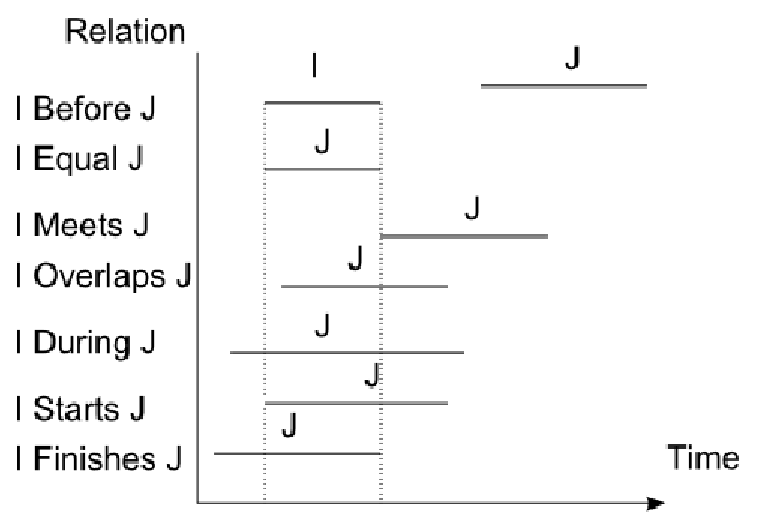
\includegraphics[width=0.8\columnwidth]{graphs/allen.eps}
   \caption{The Allen relationships between two crisp intervals $I$ and $J$.  }
   \label{fig:allen-relationships}
 \end{figure}
